%----------------------------------------------------------------------------------------------------------
% 	Copyright (c) 2009 R-forge 'distributions' Core Team, 
% 	
%	The following Sweave code is under the GNU Free Documentation License:
%      	Permission is granted to copy, distribute and/or modify this document
%      	under the terms of the GNU Free Documentation License, Version 1.3
%      	or any later version published by the Free Software Foundation;
%      	with no Invariant Sections, no Front-Cover Texts, and no Back-Cover Texts.
%
%      A copy of the license is included in the 'inst' directory of this package 
%      or on the web at http://www.gnu.org/licenses/licenses.html#FDL
%
%	After running Sweave, the following code could be compiled :
%	  - on windows with a Tex distribution such as miktex (http://miktex.org) 
%		and a front end Latex editor such as texniccenter (http://www.toolscenter.org)
%	  - on mac os with a Tex distribution such as TexLive and a front end Latex
%	  	editor such as Texshop (http://www.uoregon.edu/~koch/texshop/)
%	  - on linux with a Tex distribution such as teTex (http://www.tug.org/teTeX/)
%	  	and a front end Latex editor such as emacs (http://www.gnu.org/software/emacs/)
%
%----------------------------------------------------------------------------------------------------------

\chapter{Finite support distribution}
%%%%%%%%%%%%%%%%%%%%%%%%%%%%%%%%%%%%%%%%%%
\section{Uniform distribution}
\subsection{Characterization}
\begin{wrapfigure}{r}{0.5\textwidth}
  \vspace{-20pt}
  \begin{center}
    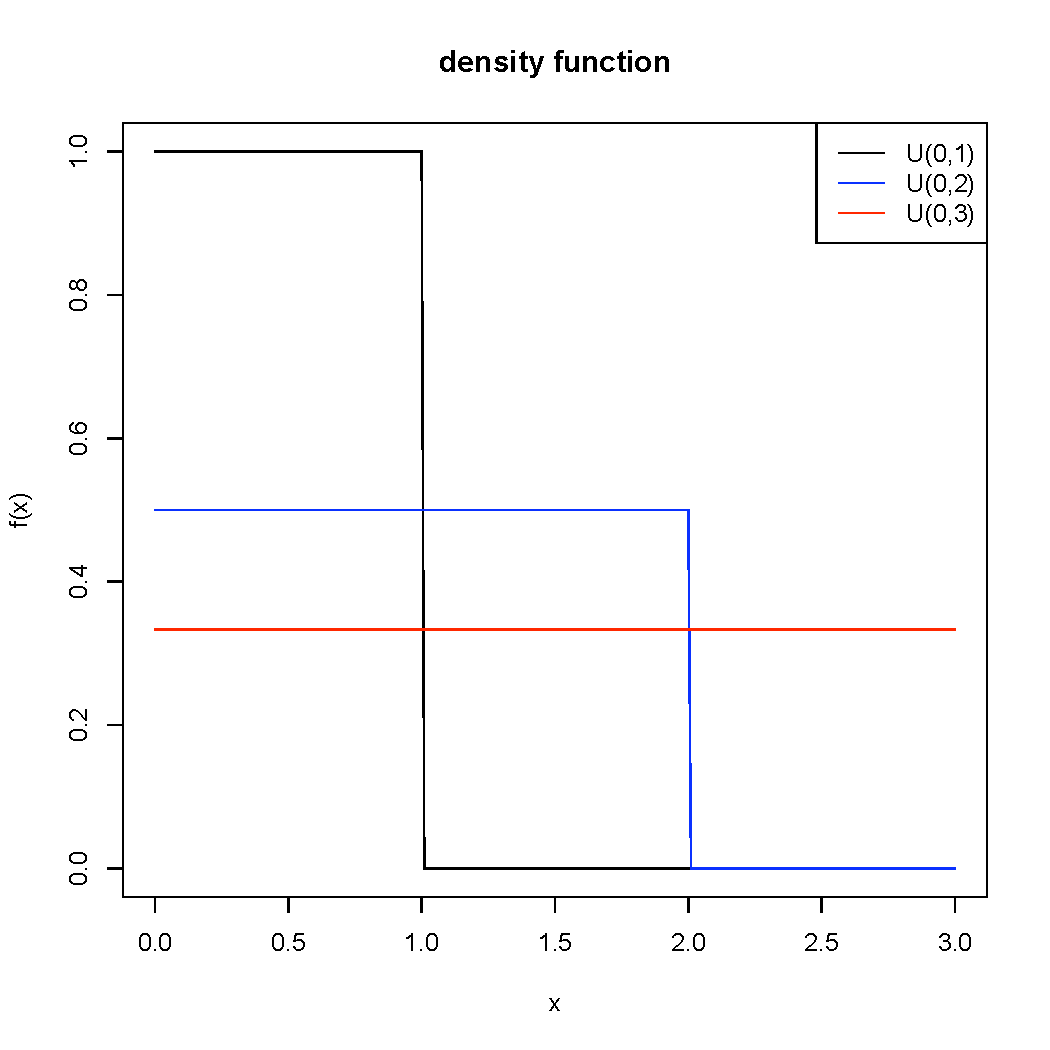
\includegraphics[width=0.48\textwidth]{img/unifzoom}
  \end{center}
  \vspace{-20pt}  
  \caption{Density function for uniform distribution}
  \vspace{-20pt}  
\end{wrapfigure}

The uniform distribution is the most intuitive distribution, its density function is 
$$
f(x) = \frac{1}{b-a},
$$
where $x\in [a,b]$ and $a<b\in \mathbb R$. So the uniform $\mathcal U(a,b)$ is only valued in $[a,b]$.
From this, we can derive the following distribution function
$$
F(x) = \left\{
\begin{array}{ll}
0 & \txtm{if} x<a\\
\frac{x-a}{b-a} & \txtm{if} a\leq x\leq b\\
1 & \txtm{otherwise}\\
\end{array}
\right. .
$$

Another way to define the uniform distribution is to use the moment generating function
$$
M(t) = \frac{e^{tb}-e^{ta}}{t(b-a)}
$$
whereas its characteristic function is 
$$
\phi(t) = \frac{e^{ibt}-e^{iat}}{i(b-a)t}.
$$

\subsection{Properties}
The expectation of a uniform distribution is $E(X) = \frac{a+b}{2}$ and its variance $Var(X)=\frac{(b-a)^2}{12}.$

If $U$ is uniformally distributed $\mathcal U(0,1)$, then $(b-a) \times U + a$ follows a uniform distribution $\mathcal U(a,b)$.

The sum of two uniform distribution does not follow a uniform distribution but a triangle distribution.

The order statistic $X_{k:n}$ of a sample of $n$ i.i.d. uniform $\mcal U(0,1)$ random variable is beta distributed $\mcal Beta(k, n-k+1)$.

Last but not least property is that for all random variables $Y$ having a distribution function $F_Y$, the random variable $F_Y(Y)$ follows a uniform distribution $\mathcal U(0,1)$. Equivalently, we get that the random variable $F_Y^{-1}(U)$ has the same distribution as $Y$ where $U\sim \mathcal U(0,1)$ and $F_Y^{-1}$ is the generalized inverse distribution function. Thus, we can generate any random variables having a distribution from the a uniform variate. This methods is called the inverse function method.


\subsection{Estimation}
For a sample $(X_i)_i$ of i.i.d. uniform variate, maximum likelihood estimators for $a$ and $b$ are respectively $X_{1:n}$ and $X_{n:n}$, where $X_{i:n}$ denotes the order statistics. But they are biased so we can use the following unbiased estimators
$$
\hat a = \frac{n}{n^2-1} X_{1:n} + \frac{1}{1-n^2}X_{n:n} \txtm{and}
\hat b = \frac{1}{1-n^2} X_{1:n} + \frac{n}{n^2-1}X_{n:n}.
$$
Finally the method of moments gives the following estimators
$$
\tilde a = \bar X_n -\sqrt{3 S_n^2} \txtm{and} \tilde b = \bar X_n +\sqrt{3 S_n^2}.
$$

\subsection{Random number generation}
Since this is the core distribution, the distribution can not be generated from another distribution. In our modern computers, we use deterministic algorithms to generate uniform variate initialized with the machine time. Generally, Mersenne-Twister algorithm (or its extensions) from \cite{matsumoto98} is implemented, cf. \cite{dutangc08} for an overview of random number generation.

\subsection{Applications}
The main application is sampling from an uniform distribution by the inverse function method.


%%%%%%%%%%%%%%%%%%%%%%%%%%%%%%%%%%%%%%%%%%
\section{Triangular distribution}
\subsection{Characterization}
\begin{wrapfigure}{r}{0.5\textwidth}
  \vspace{-20pt}
  \begin{center}
    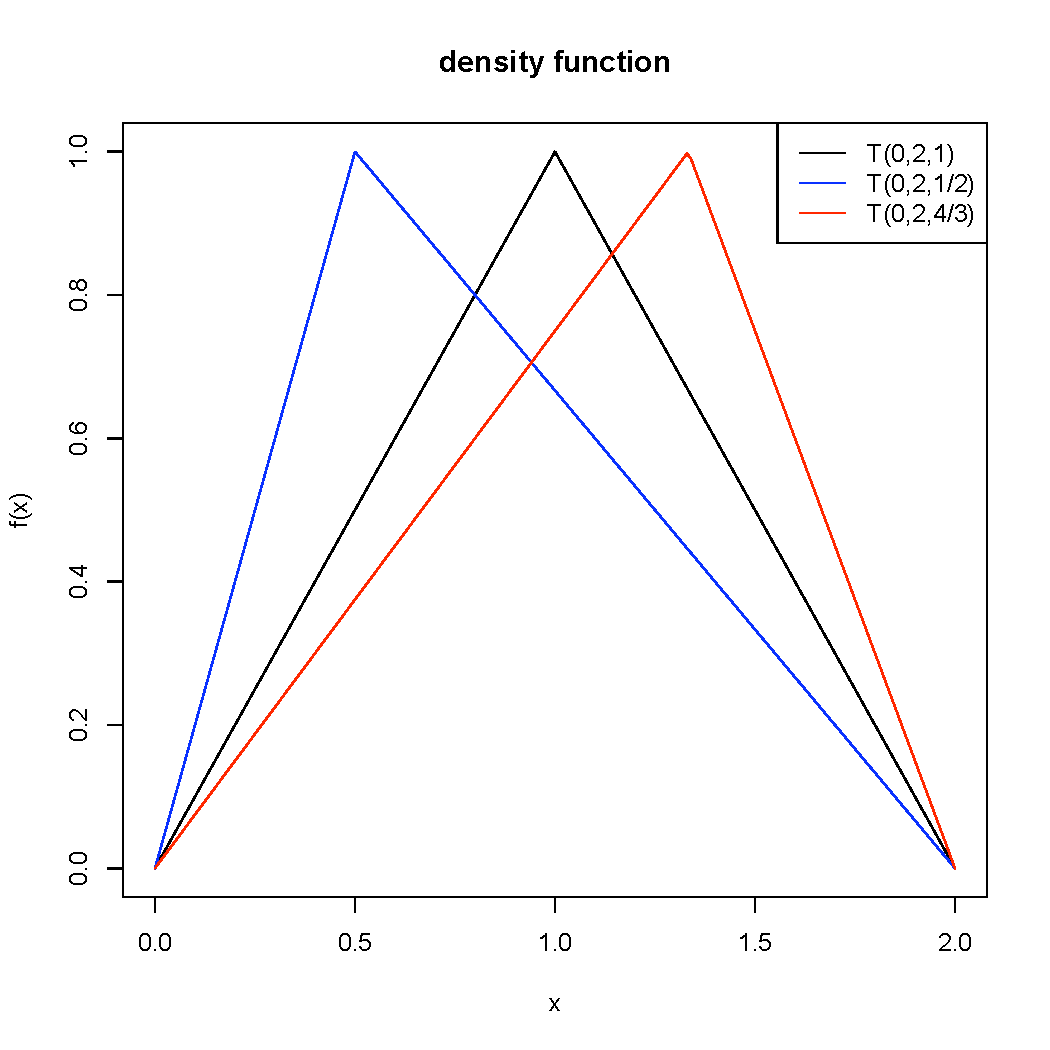
\includegraphics[width=0.48\textwidth]{img/trianglezoom}
  \end{center}
  \vspace{-20pt}  
  \caption{Density function for triangular distributions}
\end{wrapfigure}

The triangular distribution has the following density
$$
f(x) = \left\{
\begin{array}{ll}
\frac{2(x-a)}{(b-a)(c-a)} & \txtm{if} a\leq x\leq c\\
\frac{2(b-x)}{(b-a)(b-c)} & \txtm{if}c\leq x\leq b
\end{array}
\right. ,
$$
where $x\in[a,b]$, $a\in\mathbb R$, $a < b$ and $a\leq c\leq b$. The associated distribution function
is
$$
F(x) = \left\{
\begin{array}{ll}
\frac{(x-a)^2}{(b-a)(c-a)} & \txtm{if} a\leq x\leq c\\
1-  \frac{(b-x)^2}{(b-a)(b-c)} & \txtm{if}c\leq x\leq b
\end{array}
\right. .
$$

As many finite support distribution, we have a characteristic function and a moment generating function. They have the following expresion:
$$
\phi(t) = \frac{(b-c)e^{iat}-(b-a)e^{ict}}{-2(b-a)(c-a)(b-c)t^2}+\frac{-2(c-a)e^{ibt}}{(b-a)(c-a)(b-c)t^2} 
$$
and
$$
M(t) = \frac{(b-c)e^{at}-(b-a)e^{ct}}{2(b-a)(c-a)(b-c)t^2}+\frac{2(c-a)e^{bt}}{(b-a)(c-a)(b-c)t^2}.
$$



\subsection{Properties}
The expectation of the triangle distribution is $E(X) = \frac{a+b+c}{3}$ whereas its variance is $Var(X) = \frac{a^2+b^2+c^2}{18}-\frac{ab+ac+bc}{18}$.

\subsection{Estimation}
Maximum likelihood estimators for $a$, $b$, $c$ do not have closed form. But we can maximise the log-likelihood numerically. Furthermore, moment based estimators have to be computed numerically solving the system of sample moments and theoretical ones. One intuitive way to estimate the parameters of the triangle distribution is to use sample minimum, maximum and mode:
$\hat a = X_{1:n}$, $\hat b=X_{n:n}$ and $\hat c = \textrm{mode}(X_1,\dots,X_n)$, where $\textrm{mode}(X_1,\dots,X_n)$ is the middle of the interval whose bounds are the most likely order statistics.

\subsection{Random generation}
The inverse function method can be used since the quantile function has a closed form:
$$
F^{-1}(u) = \left\{
\begin{array}{ll}
a+\sqrt{u(b-a)(c-a)} & \txtm{if} 0\leq u\leq \frac{c-a}{b-a}\\
b-\sqrt{(1-u)(b-a)(b-c)} & \txtm{if} \frac{c-a}{b-a} \leq u \leq1\\
\end{array}
\right. .
$$
Thus $F^{-1}(U)$ with $U$ a uniform variable is triangular distributed.

\cite{steinkeblis} provides new kind of methods to simulate triangular variable. An algorithm for the triangular $\mcal T(0,1,c)$ distribution is provided. It can be adapted for $a,b,c$ in general. 
Let $\tilde c$ be $\frac{c-a}{b-a}$ which is in $]0,1[$. The ``minmax'' algorithm is
\begin{itemize}
\item generate $U,V$ (idependently) from a uniform distribution,
\item $X =  a+(b-a)\times\left[(1-\tilde c) \min(U,V) + \tilde c \max(U,V)\right]$.
\end{itemize}
This article also provides another method using a square root of uniform variate, which is called ``one line method'', but it is not necessary more fast if we use vector operation.

\subsection{Applications}
A typical of the triangle distribution is when we know the minimum and the maximum of outputs of an interest variable plus the most likely outcome, which represent the parameter $a, b$ and $c$. For example we may use it in business decision making based on simulation of the outcome, in project management to model events during an interval and in audio dithering.

%%%%%%%%%%%%%%%%%%%%%%%%%%%%%%%%%%%%%%%%%%%
\section{Beta type I distribution}
\subsection{Characterization}
\begin{wrapfigure}{r}{0.5\textwidth}
  \vspace{-20pt}
  \begin{center}
    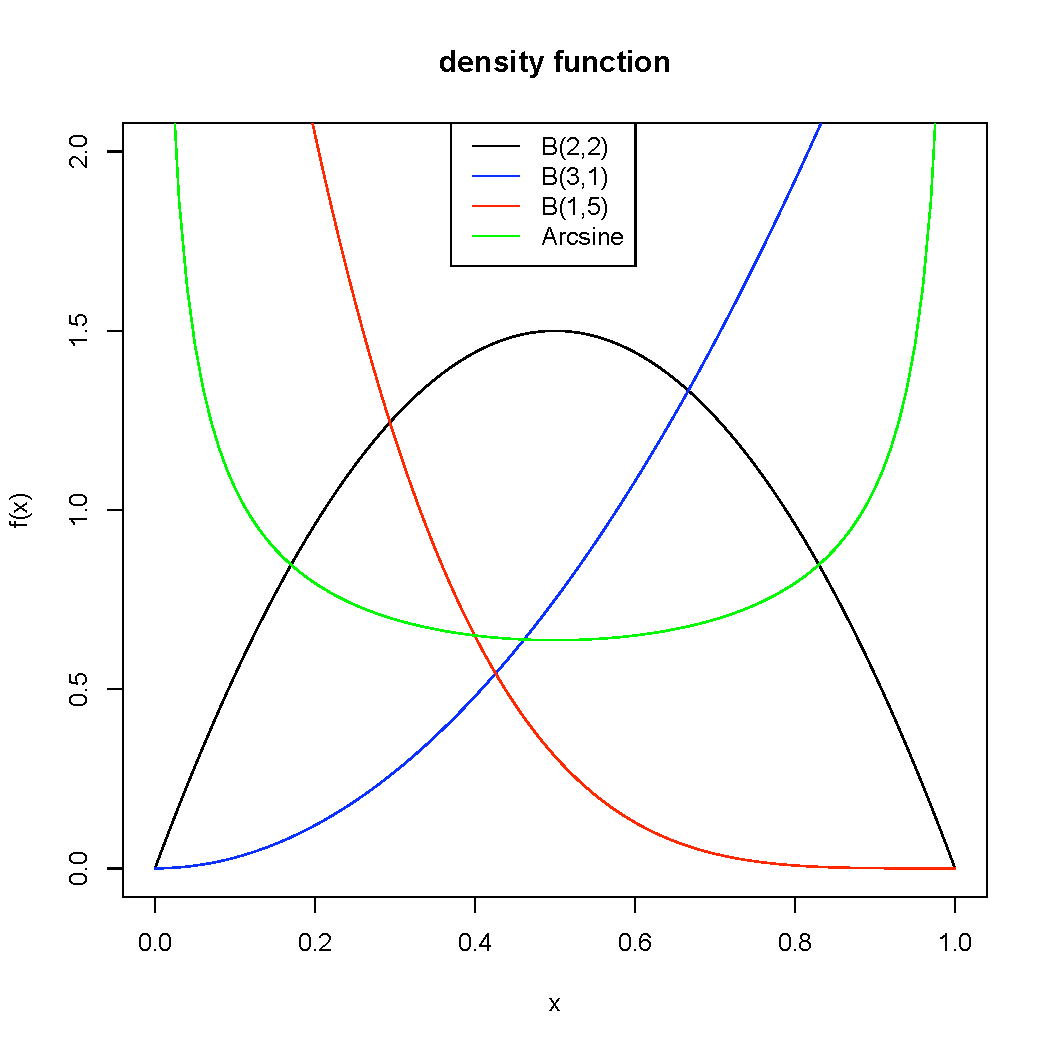
\includegraphics[width=0.48\textwidth]{img/betazoom}
  \end{center}
  \vspace{-20pt}  
  \caption{Density function for beta distributions}
\end{wrapfigure}
The beta distribution of first kind is a distribution valued in the interval $[0,1]$. Its density is defined as
$$
f(x) = \frac{x^{a-1} (1-x)^{b-1} }{\beta(a,b)},
$$
where $x\in [0,1]$, $a,b>0$ and $\beta(.,.)$ is the beta function defined in terms of the gamma function.

Since $a,b$ can take a wide range of values, this allows many different shapes for the beta density:
\begin{itemize}
\item $a=b=1$ corresponds to the uniform distribution
\item when $a,b<1$, density is U-shapped
\item when $a<1$, $b\geq 1$ or $a=1$, $b>1$, density is strictly decreasing
	\begin{itemize}
	\item for $a=1,b>2$, density is strictly convex
	\item for $a=1, b=2$, density is a straight line
	\item for $a=1, 1<b<2$, density is strictly concave
	\end{itemize}
\item when $a=1, b<1$ or $a>1, b\leq 1$, density is strictly increasing 	\begin{itemize}
	\item for $a>2,b=1$, density is strictly convex
	\item for $a=2, b=1$, density is a straight line
	\item for $1<a<2, b=1$, density is strictly concave
	\end{itemize}
\item when $a,b>1$, density is unimodal.
\end{itemize}
Let us note that $a=b$ implies a symmetric density.

From the density, we can derive its distribution function
$$
F(x) = \frac{\beta(a,b,x)}{\beta(a,b)},
$$
where $x\in [0,1]$ and $\beta(.,.,.)$ denotes the incomplete beta function. There is no analytical formula for the incomplete beta function but can be approximated numerically.

There exists a scaled version of the beta I distribution. Let $\theta$ be a positive scale parameter. The density of the scaled beta I distribution is given by
$$
f(x) = \frac{x^{a-1} (\theta-x)^{b-1} }{\theta^{a+b-1}\beta(a,b)},
$$
where $x\in [0,\theta]$. We have the following distribution function
$$
F(x) = \frac{\beta(a,b,\frac{x}{\theta})}{\beta(a,b)}.
$$

Beta I distributions have moment generating function and characteristic function expressed in terms of series:
$$
M(t)=1  +\sum_{k=1}^{+\infty} \left( \prod_{r=0}^{k-1} \frac{a+r}{a+b+r} \right) \frac{t^k}{k!}
$$
and
$$
\phi(t) = {}_1F_1(a; a+b; i\,t),
$$
where ${}_1F_1$ denotes the hypergeometric function.

\subsection{Special cases}

A special case of the beta I distribution is the arcsine distribution, when $a=b=\frac{1}{2}$. In this special case, we have
$$
f(x) = \frac{1}{\pi\sqrt{x(1-x)}},
$$
from which we derive the following distribution function
$$
F(x) = \frac{2}{\pi} \arcsin(\sqrt{x}).
$$

Another special case is the power distribution when $b=1$, with the following density
$$
f(x) = a x^{a-1}
\txtm{and}
F(x) = x^a,
$$
for $0<x<1$.

\subsection{Properties}
The moments of the beta I distribution are $E(X) = \frac{a}{a+b}$ and $Var(X)=\frac{ab}{(a+b)^2(a+b+1)}$ (and $\frac{\theta a}{a+b}$, $\frac{\theta^2ab}{(a+b)^2(a+b+1)}$ for the scaled version respectively).

Raw moments for the beta I distribution are given by
$$
E(X^r) = \frac{\Gamma(\alpha+\beta)\Gamma(\alpha+r)}{\Gamma(\alpha+\beta+r)\Gamma(\alpha)},
$$
while central moments have the following expression
$$
E\left((X-E(X))^r\right) = \left(-\frac{\alpha}{\alpha+\beta}\right)^r {}_2F_1 \left(\alpha, -r, \alpha+\beta,\frac{\alpha+\beta}{\alpha}\right).
$$

For the arcsine distribution, we have $\frac{1}{2}$ and $\frac{1}{8}$ respectively. Let us note that the expectation of a arcsine distribution is the least probable value!

Let $n$ be an integer. If we consider $n$ i.i.d. uniform $\mcal U(0,1)$ variables $U_i$, then the distribution of the maximum $\underset{1\leq i\leq n}{\max} U_i$ of these random variables follows a beta I distribution $\mcal B(n,1)$.



\subsection{Estimation}
Maximum likelihood estimators for $a$ and $b$ do not have closed form, we must solve the system
$$
\left\{
\begin{array}{l}
\frac{1}{n}\sum\limits_{i=1}^n\log(X_i) = \beta(a,b) (\psi(a+b)-\psi(a)) \\
\frac{1}{n}\sum\limits_{i=1}^n\log(1-X_i) = \beta(a,b) (\psi(a+b)-\psi(b)) \\
\end{array}
\right.
$$
numerically, where $\psi(.)$ denotes the digamma function.

Method of moments gives the following estimators
$$
\tilde a = \bar X_n \left(\frac{\bar X_n (1 - \bar X_n)}{S_n^2} - 1 \right)
\txtm{and}
\tilde b = \tilde a \frac{1-\bar X_n}{\bar X_n}.
$$

\subsection{Random generation}
NEED REFERENCE

\subsection{Applications}
The arcsine distribution (a special case of the beta I) can be used in game theory. If we have two players playint at head/tail coin game and denote by $(S_i)_{i\geq 1}$ the serie of gains of the first player for the different game events, then the distribution of the proportion of gains among all the $S_i$'s that are positive follows asymptotically an arcsine distribution.

%%%%%%%%%%%%%%%%%%%%%%%%%%%%%%%%%%%%%%%%%%
\section{Generalized beta I distribution}
\subsection{Characterization}
\begin{wrapfigure}{r}{0.5\textwidth}
  \vspace{-20pt}
  \begin{center}
    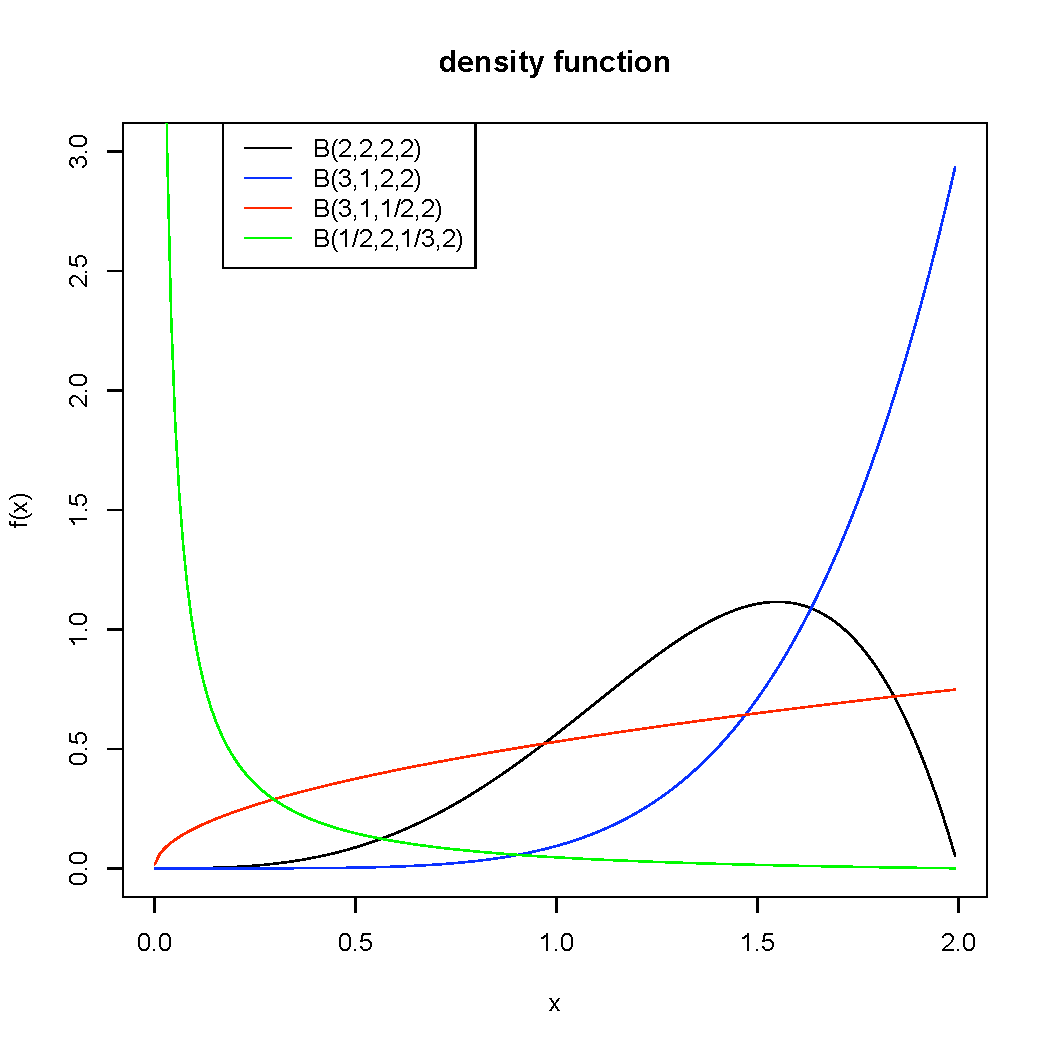
\includegraphics[width=0.48\textwidth]{img/genbetazoom}
  \end{center}
  \vspace{-20pt}  
  \caption{Density function for generalized beta distributions}
    \vspace{-20pt}  
\end{wrapfigure}

The generalized beta distribution is the distribution of the variable $\theta X^{\frac{1}{\tau}}$ when $X$ is beta distributed. Thus it has the following density
$$
f(x) = \frac{(x/\theta)^{a-1} (1-(x/\theta))^{b-1}}{ \beta(a,b)}   \frac{\tau}{x}
$$
for $0<x<\theta$ and $a, b, \tau, \theta>0$. $\theta$ is a scale parameter while $a, b, \tau$ are shape parameters.

As for the beta distribution, the distribution function is expressed in terms of the incomplete beta function
$$
F(x) = \frac{\beta(a,b,(\frac{x}{\theta})^\tau)}{\beta(a,b)},
$$
for $0<x<\theta$.

\subsection{Properties}
Moments of the generalized beta distribution are given by the formula
$$
E(X^r) = \theta^r \frac{\beta(a+\frac{r}{\tau})}{\beta(a,b)}.
$$

For $\tau=\theta=1$, we retrieve the beta I distribution.

\subsection{Estimation}
Maximum likelihood estimators as well as moment based estimators have no chance to have explicit form, but we can compute it numerically.
NEED REFERENCE

\subsection{Random generation}
NEED REFERENCE
\subsection{Applications}
NEED REFERENCE

%%%%%%%%%%%%%%%%%%%%%%%%%%%%%%%%%%%%%%%%%%
\section{Generalization of the generalized beta I distribution}
\subsection{Characterization}
A generalization of the generalized beta distribution has been studied in \cite{kotznadara}.
Its density is given by
$$
f(x) = \frac{b\beta(a,b)}{\beta(a,b+\gamma)} x^{a+b-1} {}_2F_1(1-\gamma, a, a+b,x),
$$
where $0<x<1$ and ${}_2F_1$ denotes the hypergeometric function.
Its distribution function is also expressed in terms of the hypergeometric function:
$$
F(x) = \frac{b\beta(a,b)}{(a+b)\beta(a,b+\gamma)} x^{a+b} {}_2F_1(1-\gamma, a, a+b+1,x),
$$

\subsection{Special cases}
\cite{kotznadara} list specials cases of this distribution:
If $a+b+\gamma=1$ then we get 
$$
f(x) = \frac{b\Gamma(b)x^{a+b-1}(1-x)^{-a}}{\Gamma(1-a)\Gamma(a+b)}.
$$
If $a+b+\gamma=2$ then we get
$$
f(x) = \frac{b(a+b-1)\beta(a,b)}{\beta(a,2-a)}\beta(a+b-1,1-a,x)
$$
If in addition
\begin{itemize}
\item  $a+b-1\in\mbb N$, we have
$$
f(x) = \frac{b(a+b-1)\beta(a,b)\beta(a+b-1,1-a)}{\beta(a,2-a)} \left(1- \sum_{i=1}^{a+b-1}\frac{\Gamma(i-a)}{\Gamma(1-a)\Gamma(i)} x^{i-1}(1-x)^{1-a} \right)
$$
\item  $a=1/2$ and $b=1$, we have
$$
f(x) = \frac{4}{\pi}\arctan\sqrt{\frac{x}{1-x}}
$$
\item  $a=1/2$ and $b=k\in\mbb N$, we have
$$
f(x) = \frac{k(2k-1)\beta(1/2,k)\beta(1/2,k-1/2)}{\pi}\left(\frac{2}{\pi}\arctan\sqrt{\frac{x}{1-x}} -\sqrt{x(1-x)}\sum_{i=1}^{k-1}d_i(x,k) \right)
$$
\end{itemize}
If $\gamma=0$ then, we get
$$
f(x) = b(a+b-1)(1-x)^{b-1}\beta(a+b-1,1-b,x)
$$
If in addition
\begin{itemize}
\item  $a+b-1\in\mbb N$, we have
$$
f(x) = b(a+b-1)\beta(a,b)\beta(a+b-1,1-a) \left(1- \sum_{i=1}^{a+b-1}\frac{\Gamma(i-b)}{\Gamma(1-b)\Gamma(i)} x^{i-1}(1-x)^{1-b} \right)
$$
\item $a=1$ and $b=1/2$, we have
$$
f(x) = \frac{1}{2\sqrt{1-x}}\arctan\sqrt{\frac{x}{1-x}}
$$
\item $a=k\in\mbb N$, we have
$$
f(x) = \frac{(2k-1)\beta(1/2,k-1/2)}{4\sqrt{1-x}}\left(\frac{2}{\pi}\arctan\sqrt{\frac{x}{1-x}} -\sqrt{x(1-x)}\sum_{i=1}^{k-1}d_i(x,k) \right)
$$
\end{itemize}
If $\gamma=1$, then we get a power function
$$
f(x) = (a+b)x^{a+b-1}
$$
If $a=0$, then we get a power function 
$$
f(x) = bx^{b-1}
$$
If $b=0$, then we get
$$
f(x) = \frac{\beta(a,\gamma,x)}{\beta(a,\gamma+1)}
$$
If in addition
\begin{itemize}
\item  $a\in\mbb N$, we have
$$
f(x) = \left(\frac{a}{\gamma}+1\right)\left( 1-\sum_{i=1}^a\frac{\Gamma(\gamma+i-1)}{\Gamma(\gamma)\Gamma(i)}x^{i-1}(1-x)^{\gamma} \right)
$$
\item  $\gamma\in\mbb N$, we have
$$
f(x) = \left(\frac{a}{\gamma}+1\right)\left( 1-\sum_{i=1}^a\frac{\Gamma(a+i-1)}{\Gamma(a)\Gamma(i)}x^a(1-x)^{i-1} \right)
$$
\item $a=\gamma=1/2$, we have
$$
f(x) = \frac{4}{\pi}\arctan\sqrt{\frac{x}{1-x}}
$$
\item $a=k-1/2$ and $\gamma=j-1/2$ with $k,j\in\mbb N$, we have
$$
f(x) = \left(\frac{a}{\gamma}+1\right) \left(\frac{2}{\pi}\arctan\sqrt{\frac{x}{1-x}} -\sqrt{x(1-x)}\sum_{i=1}^{k-1}d_i(x,k)+\sum_{i=1}^{j-1}c_i(x,k) \right)
$$
\end{itemize}
Where $c_i, d_i$ functions are defined by
$$
c_i(x,k) = \frac{\Gamma(k+i-1)x^{k-1/2}(1-x)^{i-1/2}}{\Gamma(k-1/2)\Gamma(i+1/2)}
$$
and
$$
d_i(x,k) = \frac{\Gamma(i)x^{i-1}}{\Gamma(i+1/2)\Gamma(1/2)}.
$$

\subsection{Properties}
Moments for this distribution are given by
$$
E(X^n) = \frac{b\beta(a,b)}{(n+a+b)\beta(a,b+\gamma)} x^{a+b} {}_3F_1(1-\gamma, a, n+a+b+1, a+b, n+a+b+1, 1),
$$
where ${}_3F_1$ is a hypergeometric function.


\subsection{Estimation}
NEED REFERENCE
\subsection{Random generation}
NEED REFERENCE
\subsection{Applications}
NEED REFERENCE

%%%%%%%%%%%%%%%%%%%%%%%%%%%%%%%%%%%%%%%%%%
\section{Kumaraswamy distribution}
\subsection{Characterization}
\begin{wrapfigure}{r}{0.5\textwidth}
  \vspace{-20pt}
  \begin{center}
    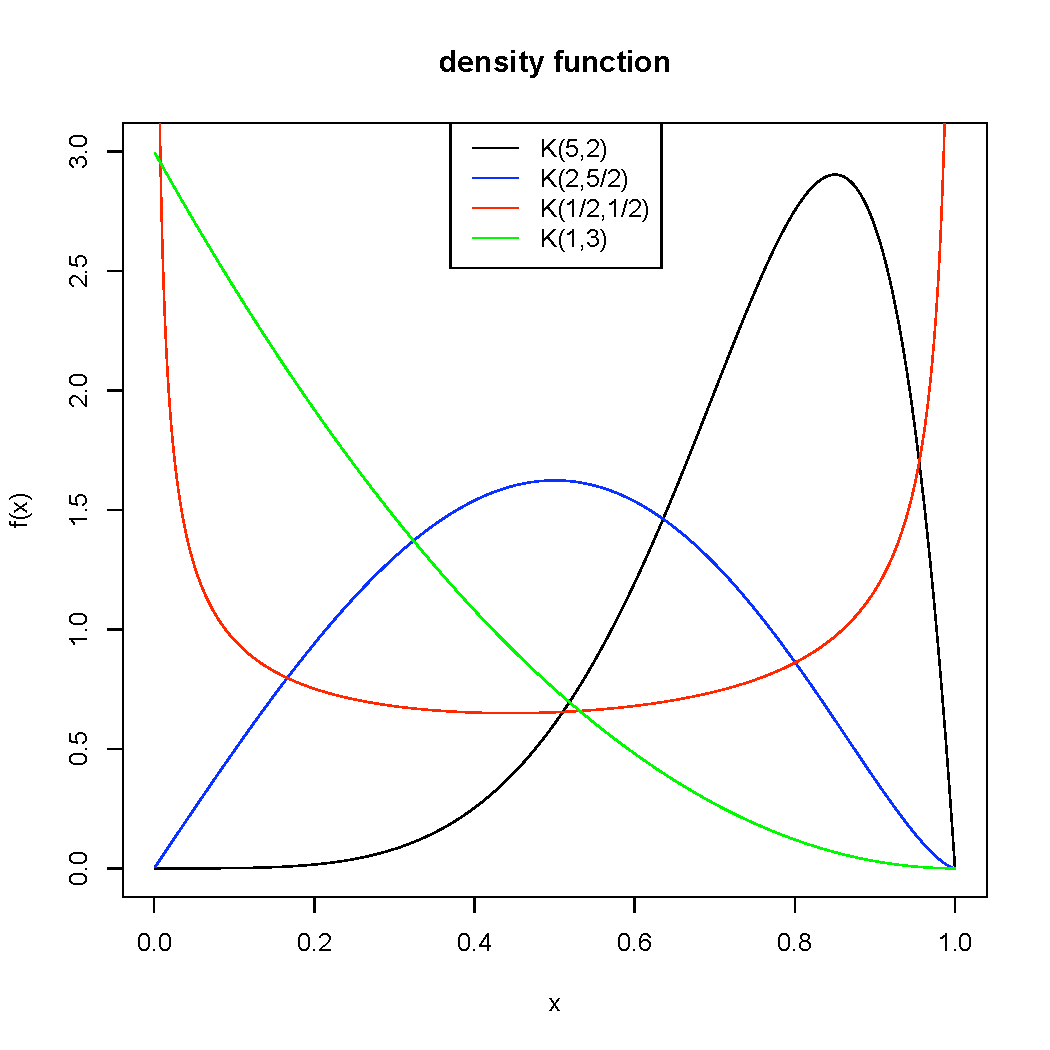
\includegraphics[width=0.48\textwidth]{img/kumarzoom}
  \end{center}
  \vspace{-20pt}  
  \caption{Density function for Kumaraswamy distributions}
\end{wrapfigure}
The Kumaraswamy distribution has the following density function
$$
f(x) = abx^{a-1}(1-x^a)^{b-1},
$$
where $x\in [0,1]$, $a,b>0$. Its distribution function is 
$$
F(x) = 1-(1-x^a)^b.
$$
A construction of the Kumaraswamy distribution use minimum/maximum of uniform samples. Let $n$
be the number of samples (each with $m$ i.i.d. uniform variate), then the distribution of the minimumm of all maxima (by sample) is a Kumaraswamy $\mcal Ku(m,n)$, which is also the distribution of one minus the maximum of all minima.

From \cite{jones}, the shapes of the density behaves as follows
\begin{itemize}
\item $a,b>1$ implies unimodal density,
\item $a>1, b\leq 1$ implies increasing density,
\item $a=b=1$ implies constant density,
\item $a\leq 1, b >1$ implies decreasing density,
\item $a,b<1$ implies uniantimodal,
\end{itemize}
which is examplified in the figure on the right.

\subsection{Properties}
Moments for a Kumaraswamy distribution are available and computable with
$$
E(X^\tau )= b\beta(1+\frac{\tau}{a},b)
$$
when $\tau > -a$ with $\beta(.,.)$ denotes the beta function. Thus the expectation of a Kumaraswamy distribution is $E(X)=\frac{b\Gamma(1+1/a)\Gamma(b)}{\Gamma(1+1/a+b)}$ and its variance $Var(X) = b\beta(1+\frac{2}{a},b) - b^2\beta^2(1+\frac{1}{a},b)$.

\subsection{Estimation}
From \cite{jones}, the maximum likelihood estimators are computable by the following procedure
\begin{enumerate}
\item solve the equation $\frac{n}{a}\left(1+\frac{1}{n}\sum_{i=1}^n \frac{\log Y_i}{1-Y_i} + \frac{ \sum_{i=1}^n \frac{Y_i\log Y_i}{1-Y_i} }{ \sum_{i=1}^n \log(1- Y_i) } \right)$ with $Y_i=X_i^a$ to find $\hat a$\footnote{the solution for this equation exists and is unique.},
\item compute $\hat b = -n\left( \sum_{i=1}^n \log(1- X_i^{\hat a}) \right)^{-1}$.
\end{enumerate}

\subsection{Random generation}
Since the quantile function is explicit
$$
F^{-1}(u) = \left(1-\left(1-u\right)^{\frac{1}{b}} \right)^{\frac{1}{a}},
$$
an inversion function method $F^{-1}(U)$ with $U$ uniformly distributed is easily computable.


\subsection{Applications}
From wikipedia, we know a good example of the use of the Kumaraswamy distribution: the storage volume of a reservoir of capacity $z_{max}$ whose upper bound is $z_{max}$ and lower bound is 0.
